

\tikzset{every picture/.style={line width=0.75pt}} %set default line width to 0.75pt        

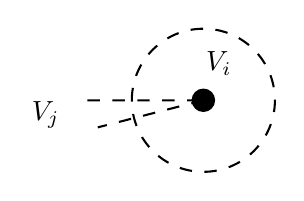
\begin{tikzpicture}[x=0.75pt,y=0.75pt,yscale=-1,xscale=1]
%uncomment if require: \path (0,507); %set diagram left start at 0, and has height of 507







%Shape: Circle [id:dp9875002869094296] 
\draw  [fill={rgb, 255:red, 0; green, 0; blue, 0 }  ,fill opacity=1 ] (88,62.15) .. controls (88,59.31) and (90.31,57) .. (93.15,57) .. controls (95.99,57) and (98.3,59.31) .. (98.3,62.15) .. controls (98.3,64.99) and (95.99,67.3) .. (93.15,67.3) .. controls (90.31,67.3) and (88,64.99) .. (88,62.15) -- cycle ;
%Straight Lines [id:da13594866224026125] 
\draw  [dash pattern={on 4.5pt off 4.5pt}]  (37.3,62.2) -- (93.15,62.15) ;
%Shape: Circle [id:dp17670679997869232] 
\draw  [dash pattern={on 4.5pt off 4.5pt}] (58.67,62.15) .. controls (58.67,43.11) and (74.11,27.67) .. (93.15,27.67) .. controls (112.19,27.67) and (127.62,43.11) .. (127.62,62.15) .. controls (127.62,81.19) and (112.19,96.62) .. (93.15,96.62) .. controls (74.11,96.62) and (58.67,81.19) .. (58.67,62.15) -- cycle ;
%Straight Lines [id:da7955461003326052] 
\draw  [dash pattern={on 4.5pt off 4.5pt}]  (93.15,62.15) -- (42.3,75.2) ;

% Text Node
\draw (93,37.4) node [anchor=north west][inner sep=0.75pt]    {$V_{i}$};
% Text Node
\draw (9,61.4) node [anchor=north west][inner sep=0.75pt]    {$V_{j}$};



% Text Node



\end{tikzpicture}
